\documentclass[aspectratio=43,10pt]{beamer}
% \documentclass[aspectratio=169,10pt]{beamer}

\usetheme[progressbar=frametitle]{metropolis}
\usepackage{appendixnumberbeamer}
\usepackage{booktabs}
% \usepackage[scale=2]{ccicons}
\usepackage{pgfplots}
\usepgfplotslibrary{dateplot}
\usepackage{xspace}
\usepackage[english,main=brazilian]{babel}
\usepackage[utf8x]{inputenc}
\usepackage[alf]{abntex2cite}
\usepackage{multirow}
\usepackage{ragged2e}
\usepackage{xspace}
\usepackage{ulem}

\usepackage{siunitx}
\sisetup{output-exponent-marker=\ensuremath{\mathrm{e}}}

\usepackage{pgfgantt}
\usepackage{algorithmic}
\usepackage[portuguese,ruled,vlined,linesnumbered]{algorithm2e}

% \usepackage{listings}
\usepackage{fancyvrb}

\title[]{Discussão de Implementação do Algoritmo MINAS}
% \subtitle{Seminários de Metodologia Científica}
\author{Luís Henrique Puhl de Souza\\
Orientador: Prof. Dr. Hermes Senger}
\institute{
Universidade Federal de São Carlos \\
Centro de Ciências Exatas e de Tecnologia \\
Departamento de Computação \\
Programa de Pós-Graduação em Ciência da Computação}
\date{\today}
% \date{Fevereiro 2020}
% \titlegraphic{\hfill\includegraphics[height=1.5cm]{logo.pdf}}

\newcommand{\nota}[1]{\hspace*{-0.5cm}\textit{{\color[rgb]{1,0,0}Nota: #1}}}

\newcommand{\mfog}{sistema M-FOG\xspace}
\newcommand{\arch}{IDSA-IoT\xspace}

\begin{document}

\maketitle

% \begin{frame}{Índice}
%   \setbeamertemplate{section in toc}[sections numbered]
%   \tableofcontents[hideallsubsections]
% \end{frame}

\section{Introdução}

\begin{frame} [fragile]{Introdução}

  Este documento tem por objetivo apresentar o algoritmo Minas e suas implementações
  guiando discussões sobre os detalhes e decisões nas implementações.

  Recorda-se que o contexto dessa discussão é o mesmo do \mfog:

\begin{itemize}%[<+- | alert@+>]

% Proposta
\item Um sistema para detecção de intrusão em Redes IoT implementando em névoa;

% hipótese
\item A hipótese do trabalho é que o algoritmo MINAS pode ser distribuído em
nós de nuvem e névoa reduzindo a latência e com pouco comprometimento na
qualidade de detecção.

\item Fundamentos
  \begin{itemize}
    \item Métodos Detecção de Novidade;
    \item Ambientes de computação Distribuída;
    \item Plataformas de processamento distribuído de fluxos.
  \end{itemize}
\end{itemize}
\end{frame}

\newcommand{\novelty}{\textit{Novelty Detection}\xspace}
\newcommand{\nd}{ND\xspace}
\newcommand{\drift}{\textit{Concept Drift}\xspace}
\newcommand{\evolution}{\textit{Concept Evolution}\xspace}

\begin{frame}[fragile]{Algoritmo MINAS}
\begin{alertblock}{Algoritmo MINAS}
  \begin{itemize}%[<+- | alert@+>]
    \item Modelo de aprendizado \textit{Offline-Online};
    \item Transformação dos dados analisados para o espaço $\mathbb{R}^d$;
    \item Modelo de classificação com \textit{Clusters};
    \item Função de classificação baseada em distância euclideana;
    \item Algoritmo de agrupamento para identificação de novos padrões;
    \item Classificação de novos padrões entre recorrência, extensão e novidade;
  \end{itemize}
\end{alertblock}
\end{frame}

\begin{frame}[fragile]{Proposta}
  \metroset{block=fill}
  \begin{block}{Proposta da Pesquisa}
    \begin{itemize}
      
      \item Implementar a distribuição do algoritmo MINAS em nuvem e névoa
      conforme arquitetura \arch;
      
      \item Paralelizar o método de classificação do algoritmo MINAS.
    \end{itemize}
  \end{block}

  \metroset{block=transparent}
  \begin{alertblock}{Metodologia}
    \begin{itemize}%[<+- | alert@+>]
      \item Plataforma de processamento distribuído;
      \item Estratégias de implementação da arquitetura \arch;
      \item Experimentação com a distribuição do algoritmo MINAS em ambientes;
      \item Métricas de qualidade de classificação para validação da implementação;
      \item Métricas de escalabilidade.
    \end{itemize}
  \end{alertblock}
\end{frame}


\newcommand{\source}{módulo auxiliar \textit{source}\xspace}
\newcommand{\sink}{módulo auxiliar \textit{sink}\xspace}

\newcommand{\offline}{módulo treinamento\xspace}
\newcommand{\classify}{módulo classificador\xspace}
\newcommand{\detector}{módulo detector de novidades\xspace}

\begin{frame}[fragile]{Proposta}

  O \mfog é dividido em 5 módulos subdivididos em 2 grupos.
  
  \begin{alertblock}{Módulos principais implementam o algoritmo MINAS}
    \begin{itemize}
      \item \offline (\textit{Training Module});
      \item \classify (\textit{Classification Module});
      \item \detector (\textit{Novelty Detection Module}).
    \end{itemize}
  \end{alertblock}
  \begin{alertblock}{Módulos auxiliares, utilizados para avaliação}
    \begin{itemize}
      \item \source (fonte);
      \item \sink (sorvedouro, consumidor final).
    \end{itemize}
  \end{alertblock}
\end{frame}

\begin{frame}[fragile]{Proposta}
  \vspace{-0.5cm}
  \begin{figure}[h]
    \centering
    \hspace*{-0.9cm}
    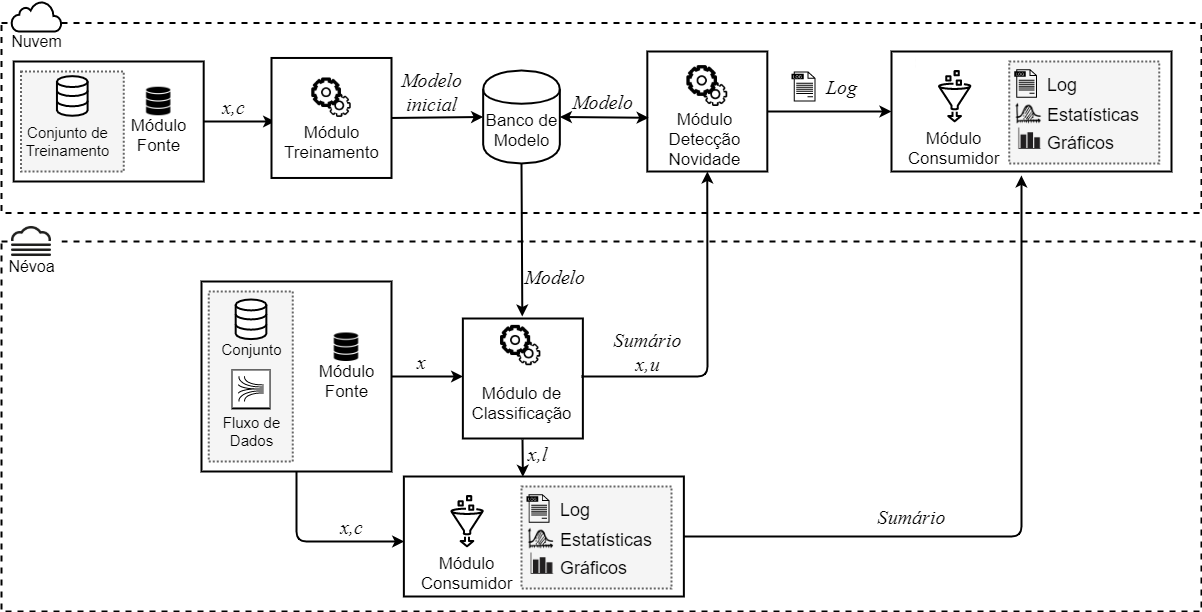
\includegraphics[width=1.1\textwidth]{../figuras/mfog-arch-v3_pt-br.png}
    \caption{Arquitetura e fluxos de dados do \mfog.}
    \label{fig:arch}
  \end{figure}
\end{frame}

\begin{frame}[fragile]{Método de Avaliação}
  \begin{alertblock}{Métricas e Ambientes}
    \begin{itemize}
      \item Métricas de qualidade de classificação:
      \begin{itemize}
        \item Avaliação do fluxo de saída do classificador;
        \item Uso de uma matriz de confusão ou erro;
        \item Taxa de desconhecidos;
        \item Macro F-score;
      \end{itemize}
    \end{itemize}
  \end{alertblock}

  \begin{columns}[T,onlytextwidth]
    \column{0.5\textwidth}
    \begin{equation*}
      \mathbf{E}_n = \begin{pmatrix}
        e_{1,1} & e_{1,2} & \cdots & e_{1,J} \\
        e_{2,1} & e_{2,2} & \cdots & e_{2,J} \\
        \vdots  & \vdots  & \ddots & \vdots  \\
        e_{M,1} & e_{M,2} & \cdots & e_{M,J} 
      \end{pmatrix}
    \end{equation*}

    % 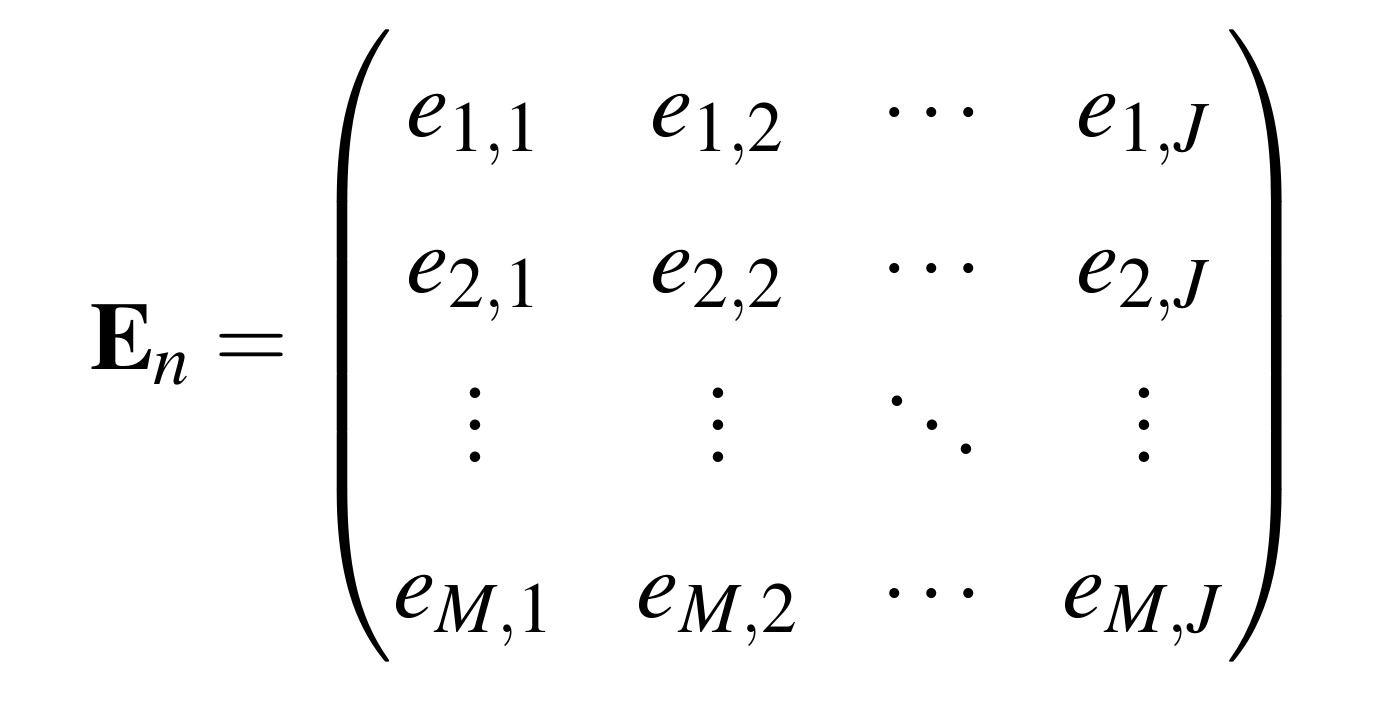
\includegraphics[width=0.9\textwidth]{figuras/eq-matrix.png}
    
    \column{0.5\textwidth}
    
    % 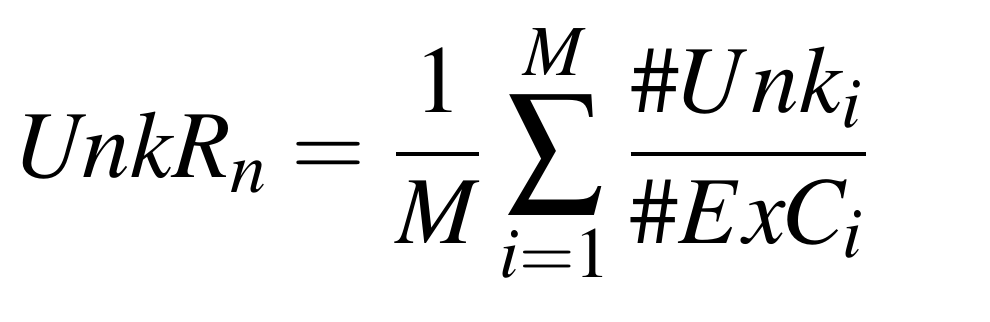
\includegraphics[width=0.9\textwidth]{figuras/eq-unk.png}
    % 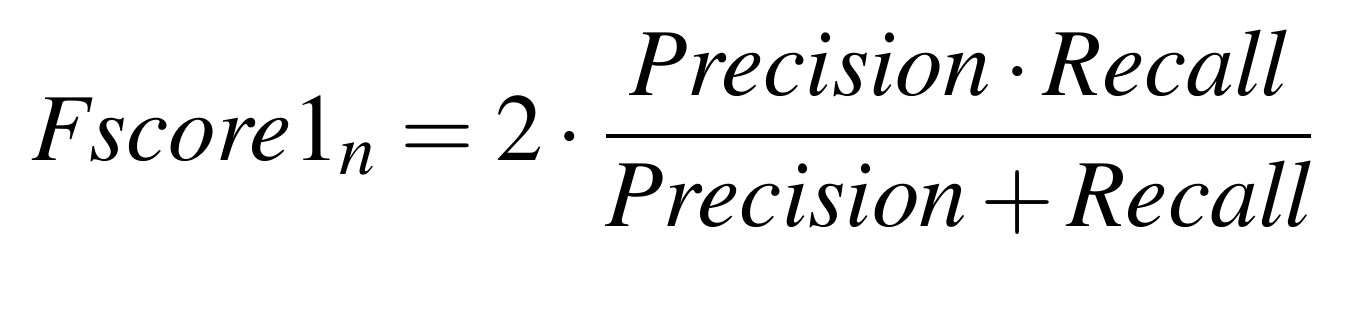
\includegraphics[width=0.9\textwidth]{figuras/eq-fscore1.png}
    
    \begin{equation*}
        \mathit{UnkR}_n      = \frac{1}{M} \sum_{i=1}^{M} \frac{\#Unk_i}{\#ExC_i} \\
        \mathit{Fscore}1_n   = 2 \cdot \frac{
          \mathit{Precision} \cdot \mathit{Recall}
          }{
            \mathit{Precision} +\mathit{Recall}
          }
    \end{equation*}
  \end{columns}
\end{frame}

% \begin{frame}[fragile]{Método de Avaliação}

%   Métricas de referência
%   \vspace{0.5cm}
  
%   \includegraphics[width=0.9\textwidth]{ref/Faria2015-CER-UnkR.png}
% \end{frame}

\begin{frame}[fragile]{Método de Avaliação}
  \begin{alertblock}{Métricas e Ambientes}
    \begin{itemize}
      \item Métricas de escalabilidade:
      \begin{itemize}
        \item Número e tipo de processadores;
        \item Uso de memória;
        \item Tempo de processamento;
        \item Taxa de eventos;
        \item Latência entre a produção e classificação.
      \end{itemize}
      \item Ambientes de teste:
      \begin{itemize}
        \item Computador Pessoal (para desenvolvimento);
        \item Nuvem UFSCar;
        \item Nevoa composta de SBC (\textit{Sigle Board Computer}) ARM 4 núcleos;
      \end{itemize}
    \end{itemize}
  \end{alertblock}
\end{frame}


\section{Resultados Preliminares}
\begin{frame}[fragile]{Resultados Preliminares}

  \begin{alertblock}{Primeira Implementação com \textit{Python} e \textit{Apache Kafka}}
    \begin{itemize}%[<+- | alert@+>]
      \item \textit{Python} é acessível e fornece bibliotecas diversas;
      \item \textit{Apache Kafka} é um sistema de mensagens distribuído;
      \begin{itemize}
        \item Interface de programação com cliente produtor e consumidor;
        \item Mensagens organizadas em tópicos que são distribuídos em partições;
      \end{itemize}
      \item A hipótese de que a carga seria distribuída entre os consumidores,
      uma vez que o consumidor pode selecionar uma partição para leitura;
      \item Em experimento com um produtor, 8 partições e 8 consumidores,
      observou-se que um consumidor processava a maior parte das mensagens,
      poucos consumidores recebiam algumas mensagens e a maioria dos consumidores
      não recebia mensagem alguma.
    \end{itemize}
  \end{alertblock}
\end{frame}

\begin{frame}[fragile]{Resultados Preliminares}
  \begin{alertblock}{Segunda Implementação com \textit{Apache Flink}}
    \begin{itemize}%[<+- | alert@+>]
      \item Implementação escrita em Scala ou Java;
      \item Processamento de fluxos \textit{Stateful};
      \item Falta de bibliotecas que distribuam algoritmos base como \textit{K-means};
      \item Ambiente de execução (\textit{Flink Cluster}) consome mais memória do
      que disponível no \textit{hardware};
      \item Tempo de execução não foi melhor que a implementação original mesmo
      sem o trecho de detecção de novidades;
    \end{itemize}
  \end{alertblock}
\end{frame}

\begin{frame}[fragile]{Resultados Preliminares}
  \begin{alertblock}{Terceira Implementação com \textit{OpenMPI}}
    \begin{itemize}%[<+- | alert@+>]
      \item Implementação escrita em C;
      \item Versão serial e versão paralela e distribuída com \textit{MPI};
      \item Reimplementação de algoritmos base como \textit{K-means};
      \item Sistema \textit{M-FOG} em desenvolvimento, atualmente na fase de
      validação através das métricas de qualidade de classificação.
      \begin{itemize}
        \item Diferença entre os modelos iniciais gerados pelo algoritmo \textit{K-means};re
        \item Diferença na matriz de confusão resultante da avaliação dos fluxos de saída;
      \end{itemize}
    \end{itemize}
  \end{alertblock}
\end{frame}

\begin{frame}[fragile]{Resultados Preliminares}
  \begin{alertblock}{Terceira Implementação com \textit{OpenMPI}}
    \includegraphics[width=1\textwidth]{ref/eval/speeup-chart.png}
  \end{alertblock}
\end{frame}

\begin{frame}[fragile]{Resultados Preliminares}
  \begin{alertblock}{Desafios Passados}
    % Desafio, resposta, justificativa
    % Artigo para setembro ou outubro.
    % Revisão dos valores da avaliação
    \begin{itemize}
      \item \sout{Diferença entre \texttt{double} e \texttt{float};}
        Use Float, diferença para o dataset pequena, economize os bits.
      \item \sout{Formato do fluxo de saída;}
        Estrutura de dados X;
      \item \sout{Tratamento de exemplos com etiqueta \textit{desconhecido} utilizados para atualização do modelo;}

      \item \sout{Diferença entre incluir ou não a borda do cluster;}
      \begin{itemize}
        \item Usar desvio padrão na classificação;
        \item Usar máximo após ND para buffer de desconhecidos;
      \end{itemize}
      \item \sout{Definição de raio;}
    \end{itemize}
  \end{alertblock}
\end{frame}
\begin{frame}[fragile]{Resultados Preliminares}
  \begin{alertblock}{Desafios Atuais}
    \begin{itemize}
      \item Distribuição e paralelização para minimização de latência entre
      novo item no fluxo e sua classificação:
      \begin{itemize}
        \item Tempo de passagem da instancia pelo classificador;
        \item Volume máximo do sistema;
        \item Diferenças de precisão de acordo com a carga;
      \end{itemize}
      \item Detecção de novidades e manutenção de modelo em ambiente distribuído:
      \begin{itemize}
        \item Mecanismo de ND local (síncrono) vs nuvem quanto à atraso de definição de modelo;
        \item Mecanismo de esquecimento local vs global (modelo único ou por nó);
        \item Atraso na reclassificação dos desconhecidos;
      \end{itemize}
    \end{itemize}
  \end{alertblock}
\end{frame}

% ------------------------------------------------------------------------------

\section{Notas de Implementação}

\begin{frame}[fragile]{Algoritmo MINAS}
  \begin{alertblock}{Outras abordagens e implementações}
    \begin{itemize}%[<+- | alert@+>]
      \item FuzzyND por Da Silva 2018;
      \item Minas-LC e Minas-BR por Costa 2019;
      \item Implementação em Java por Douglas (douglas.m.cavalcanti@gmail.com) em Jul 2 09:37:42 2019
      \item Implementação em Python por Vitor Sexto Bernardes (vitorsb@gmail.com) em May 11 23:51:09 2020
    \end{itemize}
  \end{alertblock}
\end{frame}

% \begin{frame}[fragile]{Algoritmo MINAS}
%   \begin{alertblock}{Parâmetros}
%     \includegraphics[width=1\textwidth]{ref/Faria2015-parameters.png}
%   \end{alertblock}
% \end{frame}

\begin{frame}[fragile]{Implementação referência}
  \begin{alertblock}{Parâmetros}
    % \includegraphics[width=1\textwidth]{ref/MINAS.java-params.png}
    \begin{Verbatim}[fontsize=\footnotesize]
class br.ufu.noveltydetection.minas.MinasOg with
	filenameOffline = datasets/training.csv
	filenameOnline = datasets/test.csv

	outputDirectory = out/minas-og//2020-07-20T12-18-21.758/
	algClusteringOff = kmeans
	algClusteringOnl = kmeans

	threshold = 2.0
	flagEvaluationType = 1
	thresholdForgettingPast = 10000
	numMicro = 100
	flagMicroClusters = true

	minExCluster = 20
	validationCriterion = dec

	skipNd = false
    \end{Verbatim}
  \end{alertblock}
\end{frame}
\begin{frame}[fragile]{Nova Implementação}
  \begin{alertblock}{Parâmetros}
    % \includegraphics[width=1\textwidth]{ref/MFOG-params.png}
    \begin{Verbatim}[fontsize=\small]
params->kParam = 100;
params->dimension = 22;
params->noveltyThreshold = 2;
params->minExCluster = 20;
params->maxUnkSize = params->kParam * params->minExCluster;
params->thresholdForgettingPast = 10000;
    \end{Verbatim}
  \end{alertblock}
\end{frame}

% \begin{frame}[fragile]{Algoritmo MINAS}
%   \begin{alertblock}{Fase offline}
%     \includegraphics[width=1.1\textwidth]{ref/Faria2015-Alg1-Off.png}
%   \end{alertblock}
% \end{frame}

% \begin{frame}[fragile]{Algoritmo MINAS}
%   \begin{alertblock}{Final da fase offline, inicio da fase online}
%     \begin{quotation}
    
%       [\dots] N number of examples, LS linear sum of the examples, SS squared sum of the
%       elements and T timestamp of the arrival of the last example classified in
%       this micro-cluster.

%       [\dots]
%       After the execution of the clustering algorithm, each micro-cluster is
%       represented by \alert{four components (N, LS, SS and T)}.
      
%       [\dots]
%       MINAS uses these measures to classify new examples. For such, it computes
%       the distance between a new example and the closest centroid. If this
%       distance is less than the micro-cluster radius, the example is classified
      
%       [\dots]
%       MINAS calculates the \alert{radius of a micro-cluster as the standard
%       deviation} of the distance between the examples and the centroid, multiplied
%       by a \alert{factor f}.
    
%     \end{quotation}
%   \end{alertblock}
% \end{frame}

% \begin{frame}[fragile]{Implementação referência}
%   \begin{alertblock}{Fase Offline, definição de raio}
%     \includegraphics[width=1\textwidth]{ref/MINAS.java-createKMeans.png}
    
%     Detalhe:
%     \includegraphics[width=1\textwidth]{ref/MINAS.java-createKMeans-detail.png}
%   \end{alertblock}
% \end{frame}
% \begin{frame}[fragile]{Implementação referência}
%   \begin{alertblock}{Fase Offline, definição de raio}
%     \includegraphics[width=1\textwidth]{ref/MINAS.java-Kmeans.png}
%   \end{alertblock}
% \end{frame}
% \begin{frame}[fragile]{Implementação referência}
%   \includegraphics[width=1\textwidth]{ref/MINAS.java-Kmeans-radius2.png}
% \end{frame}


% \begin{frame}[fragile]{Algoritmo MINAS}
%   \begin{alertblock}{Fase online}
%     \includegraphics[width=1\textwidth]{ref/Faria2015-Alg2-On.png}
%   \end{alertblock}
% \end{frame}

% \begin{frame}[fragile]{Implementação referência}
%   \begin{alertblock}{Fase online}
%     \includegraphics[width=1\textwidth]{ref/MINAS.java-identify.png}
%   \end{alertblock}
% \end{frame}

% \begin{frame}[fragile]{Nova Implementação}
%   \begin{alertblock}{Fase online}
%     \includegraphics[width=1\textwidth]{ref/MFOG-identify.png}
%   \end{alertblock}
% \end{frame}

% \begin{frame}[fragile]{Algoritmo MINAS}
%   \begin{alertblock}{Fase online, Detecção de novidades}
%     \includegraphics[width=1\textwidth]{ref/Faria2015-Alg3-ND.png}
%   \end{alertblock}
% \end{frame}

% \begin{frame}[fragile]{Implementação referência}
%   \begin{alertblock}{Output Stream}
%     \includegraphics[width=1\textwidth]{ref/MINAS.java-outstream.png}
%   \end{alertblock}
% \end{frame}

% \begin{frame}[fragile]{Nova Implementação}
%   \begin{alertblock}{Output Stream}
%     \includegraphics[width=1\textwidth]{ref/MFOG-outstream.png}
%   \end{alertblock}
% \end{frame}

% ------------------------------------------------------------------------------

\begin{frame}[fragile]{Implementação Referência e Avaliação de Referência}
  A implementação de referência gera um arquivo (fluxo) de saída e arquivo de
  matriz de confusão.

  Além disso é gerado um gráfico das métricas (\textit{Err, FNew, Mnew}) calculadas para cada item do fluxo.
\end{frame}

\begin{frame}[fragile]{Implementação Referência e Avaliação de Referência}
  \begin{alertblock}{Reference Output Stream, Reference Evaluation}
    \includegraphics[width=1\textwidth]{ref/MINAS.java-graph.png}
  \end{alertblock}
\end{frame}

\begin{frame}[fragile]{Implementação Referência e Avaliação de Referência}
  \begin{alertblock}{Matriz de confusão gerada pela Implementação referência}
    % \begin{tabular}{c|c|c|c|c|c|c|c|c|c|c|c|c|c|c}
    %   & C N       & N 1   & N 2   & N 3   & N 4   & N 5   & N 6   & N 7   & N 8   & N 9   & N 10  & N 11  & N 12  & Unk   \\
    %   \hline
    %   C N   & 199263    & 0     & 79    & 44    & 0     & 0     & 0     & 229   & 181   & 826   & 5088  & 289   & 0     & 279   \\
    %   C A   & 439530    & 123   & 145   & 368   & 8     & 52    & 165   & 1     & 1046  & 2133  & 3467  & 71    & 26    & 44    \\
    % \end{tabular}
    \vspace{0.5em}
    
    \begin{columns}[T,onlytextwidth]
      \column{0.5\textwidth}
      \small{
      \begin{tabular}{ l| r| r }
                       & \textbf{C N} & \textbf{C A}\\ \hline \hline
        \textbf{C N }  & $199263$    & $439530$    \\ \hline
        \textbf{N 1 }  & $0$         & $123$       \\ \hline
        \textbf{N 2 }  & $79$        & $145$       \\ \hline
        \textbf{N 3 }  & $44$        & $368$       \\ \hline
        \textbf{N 4 }  & $0$         & $8$         \\ \hline
        \textbf{N 5 }  & $0$         & $52$        \\ \hline
        \textbf{N 6 }  & $0$         & $165$       \\ \hline
        \textbf{N 7 }  & $229$       & $1$         \\ \hline
        \textbf{N 8 }  & $181$       & $1046$      \\ \hline
        \textbf{N 9 }  & $826$       & $2133$      \\ \hline
        \textbf{N 10}  & $5088$      & $3467$      \\ \hline
        \textbf{N 11}  & $289$       & $71$        \\ \hline
        \textbf{N 12}  & $0$         & $26$        \\ \hline
        \textbf{Unk }  & $279$       & $44$        \\
      \end{tabular}
      }

      \column{0.5\textwidth}
      Aplicando a técnica de associação de etiquetas à classes descrita em \citeonline{Faria2016minas},
      tem-se que $208935$ itens foram etiquetados corretamente (\textit{true positive}).
      Portanto a \textsl{taxa de acerto} é $208935 / 653457 = 0.319737948$.
    \end{columns}
  \end{alertblock}
\end{frame}

% ------------------------------------------------------------------------------

\begin{frame}[fragile]{Implementação de Referência e Nova Avaliação}
  O fluxo de saída da implementação de referência pode ser consumido pelo módulo
  de avaliação da nova implementação (\mfog).
\end{frame}

\begin{frame}[fragile]{Implementação de Referência e Nova Avaliação}
  \begin{alertblock}{Fluxo de saída Original, Grafico da Nova Avaliação}
    \includegraphics[width=1\textwidth]{ref/MINAS.java-outstream-results-hits.png}
  \end{alertblock}
\end{frame}

\begin{frame}[fragile]{Implementação de Referência e Nova Avaliação}
  \begin{alertblock}{Matriz de confusão e avaliação, Fluxo de saída Original}
    % \includegraphics[width=1\textwidth]{ref/eval/MINAS.java-conf_mat.png}
    \hspace{0.5em}
    
    \begin{columns}[T,onlytextwidth]
      \column{0.5\textwidth}
      \footnotesize{
      \begin{tabular}
        { l                     | r          | r           }
        \textbf{Classes (act)}  & \textbf{A} & \textbf{N}  \\% assigned    hits          og_labels
        \textbf{Labels (pred)}  &            &             \\
        \hline
        \hline \textbf{-}       &   $3774$    &   $8206$  \\% -              0               [Unk]
        \hline \textbf{1}       &    $123$    &      $0$  \\% A            123          [ExtNov 1]
        \hline \textbf{10}      &   $2489$    &   $4066$  \\% N           4066   [ExtNov 10, N 10]
        \hline \textbf{11}      &     $71$    &    $289$  \\% N            289   [ExtNov 11, N 11]
        \hline \textbf{12}      &     $26$    &      $0$  \\% A             26   [N 12, ExtNov 12]
        \hline \textbf{2}       &    $145$    &     $79$  \\% A            145          [ExtNov 2]
        \hline \textbf{3}       &    $368$    &     $44$  \\% A            368          [ExtNov 3]
        \hline \textbf{4}       &      $8$    &      $0$  \\% A              8          [ExtNov 4]
        \hline \textbf{5}       &     $52$    &      $0$  \\% A             52          [ExtNov 5]
        \hline \textbf{6}       &    $165$    &      $0$  \\% A            165     [N 6, ExtNov 6]
        \hline \textbf{7}       &      $1$    &    $229$  \\% N            229          [ExtNov 7]
        \hline \textbf{8}       &   $1046$    &    $181$  \\% A           1046     [N 8, ExtNov 8]
        \hline \textbf{9}       &    $161$    &    $154$  \\% A            161               [N 9]
        \hline \textbf{N}       & $438750$    & $193030$  \\% N         193030     [C N, ExtCon N]
      \end{tabular}
      }
      \column{0.5\textwidth}
      
      \footnotesize{
      \begin{tabular}
        { l                     | r                 r             }
        \textbf{Métrica}        & \textbf{Valor}  &               \\ \hline
        \hline Total examples   & $653457$        &               \\
        \hline Total matches    & $653457$        &               \\
        \hline Hits             & $199708$        & $0.30561766$  \\
        \hline Misses           & $441769$        & $0.67604907$ \\
        \hline Unknowns         & $11980$         & $0.01833326$ \\
        \hline Unk. reprocessed & $0$             & $0.00000000$ \\

      \end{tabular}
      }

    \end{columns}
  \end{alertblock}
\end{frame}

% ------------------------------------------------------------------------------

\begin{frame}[fragile]{Implementação de Referência e Nova Avaliação}
  Além do consumo do fluxo com formato original, foi adicionado à implementação
  de referência o passo de reprocessamento e saída no novo formato.
\end{frame}

\begin{frame}[fragile]{Implementação de Referência e Nova Avaliação}
  \begin{alertblock}{New Format, Reference Output Stream, Evaluation}
    \includegraphics[width=1\textwidth]{ref/MINAS.java-outstream-hits.png}
  \end{alertblock}
\end{frame}

\begin{frame}[fragile]{Implementação referência}
  \begin{alertblock}{Matriz de confusão e avaliação, Novo formato Fluxo de saída}
    % \includegraphics[width=1\textwidth]{ref/eval/MINAS.java-conf_mat.png}
    \hspace{0.5em}
    
    \begin{columns}[T,onlytextwidth]
      \column{0.5\textwidth}
      \footnotesize{
      \begin{tabular}
        { l                     | r          | r           }%| c                 | c }
        \textbf{Classes (act)}  & \textbf{A} & \textbf{N}  \\ %& \textbf{assigned} & \textbf{hits} \\
        \textbf{Labels (pred)}  &            &             \\ %&                   &               \\
        % Classes (act) & A     & N   & assigned  & hits  \\
        % Labels (pred) &       &     &           &       \\
        \hline
        \hline \textbf{-}       &   $3774$   &   $8206$   \\ % &   -                &       0 \\
        \hline \textbf{1}       &    $123$   &      $0$   \\ % &   A                &     123 \\
        \hline \textbf{10}      &   $3520$   &   $5130$   \\ % &   N                &    5130 \\
        \hline \textbf{11}      &     $71$   &    $289$   \\ % &   N                &     289 \\
        \hline \textbf{12}      &     $26$   &      $0$   \\ % &   A                &      26 \\
        \hline \textbf{2}       &    $152$   &     $82$   \\ % &   A                &     152 \\
        \hline \textbf{3}       &    $368$   &     $44$   \\ % &   A                &     368 \\
        \hline \textbf{4}       &      $8$   &      $0$   \\ % &   A                &       8 \\
        \hline \textbf{5}       &     $82$   &      $1$   \\ % &   A                &      82 \\
        \hline \textbf{6}       &    $165$   &      $0$   \\ % &   A                &     165 \\
        \hline \textbf{7}       &      $8$   &    $396$   \\ % &   N                &     396 \\
        \hline \textbf{8}       &   $1054$   &    $183$   \\ % &   A                &    1054 \\
        \hline \textbf{9}       &    $161$   &    $154$   \\ % &   A                &     161 \\
        \hline \textbf{N}       & $441395$   & $199715$   \\ % &   N                &  199715 \\
      \end{tabular}
      }
      \column{0.5\textwidth}
      
      \footnotesize{
      \begin{tabular}
        { l                     | r                 r             }
        \textbf{Métrica}        & \textbf{Valor}  &               \\ \hline
        \hline Total examples   & $653457$        &               \\
        \hline Total matches    & $665107$        &               \\
        \hline Hits             & $207669$        & $0.31223397$  \\
        \hline Misses           & $445458$        & $0.66975389$  \\
        \hline Unknowns         & $11980$         & $0.01801214$  \\
        \hline Unk. reprocessed & $11650$         & $0.97245409$  \\
      \end{tabular}
      }

    \end{columns}
  \end{alertblock}
\end{frame}

% ------------------------------------------------------------------------------

\begin{frame}[fragile]{Implementação \textit{Baseline} e Nova Avaliação}
  Implementação serial, não distribuída, do algorítmo MINAS em C que serve de
  base (biblioteca) para a implementação \mfog e para cálculo de speed-up.
\end{frame}

\begin{frame}[fragile]{Implementação \textit{Baseline} e Nova Avaliação}
  \begin{alertblock}{Baseline Output Stream, Evaluation}
    \includegraphics[width=1\textwidth]{ref/baseline-hits.png}
  \end{alertblock}
\end{frame}

\begin{frame}[fragile]{Implementação \textit{Baseline} e Nova Avaliação}
  \begin{alertblock}{Matriz de confusão e avaliação, Novo formato Fluxo de saída}
    % \includegraphics[width=1\textwidth]{ref/eval/MINAS.java-conf_mat.png}
    \hspace{0.5em}
    
    \begin{columns}[T,onlytextwidth]
      \column{0.5\textwidth}
      \footnotesize{
      \begin{tabular}
        { l                     | r          | r           }
        \textbf{Classes (act)}  & \textbf{A} & \textbf{N}  \\
        \textbf{Labels (pred)}  &            &             \\\hline
        \hline \textbf{-}       & $10263$   &  $3122$   \\% -       0
        \hline \textbf{0}       & $1798$    &  $48$     \\% A    1798
        \hline \textbf{1}       & $315$     &  $0$      \\% A     315
        \hline \textbf{2}       & $1098$    &  $156$    \\% A    1098
        \hline \textbf{3}       & $0$       &  $318$    \\% N     318
        \hline \textbf{4}       & $1510$    &  $20$     \\% A    1510
        \hline \textbf{5}       & $2$       &  $53$     \\% N      53
        \hline \textbf{6}       & $1560$    &  $2$      \\% A    1560
        \hline \textbf{7}       & $31$      &  $0$      \\% A      31
        \hline \textbf{8}       & $31$      &  $3$      \\% A      31
        \hline \textbf{9}       & $58$      &  $3$      \\% A      58
        \hline \textbf{N}       & $440712$  &  $205476$ \\% N  205476
      \end{tabular}
      }
      \column{0.5\textwidth}
      
      \footnotesize{
      \begin{tabular}
        { l                     | r                 r             }
        \textbf{Métrica}        & \textbf{Valor}  &               \\ \hline
        \hline Total examples   & $653457$        &               \\
        \hline Total matches    & $666579$        &               \\
        \hline Hits             & $212248$        & $0.31841387$  \\
        \hline Misses           & $440946$        & $0.66150599$  \\
        \hline Unknowns         & $13385$         & $0.02008014$  \\
        \hline Unk. reprocessed & $13122$         & $0.98035114$  \\
      \end{tabular}
      }

      \begin{Verbatim}[fontsize=\small]
        k=100; radiusF = 0.25;
        minExamplesPerCluster = 20;
        noveltyF = 1.4
      \end{Verbatim}

    \end{columns}
  \end{alertblock}
\end{frame}

% ------------------------------------------------------------------------------

\begin{frame}[fragile]{Implementação Referência \textit{versus} Baseline}
  \begin{alertblock}{Matriz de confusão e avaliação na Referência \textit{versus} Avaliação \mfog}
    \hspace{0.5em}

    Nota-se que como o novo método de avaliação utiliza o fluxo de saída do algoritmo,
    as métricas tem valores semelhantes mas não idênticos.
    
    Em especial, a soma de todas as células da matriz de confusão na referência é de $653457$
    (contagem de itens no fluxo de entrada)
    e na avaliação atual (\mfog) é de $665107$ (contagem de itens no fluxo de saída).
    
    O mesmo acontece no número de acertos:
    Na referência $208935$ com taxa $0.319737948$ e na avaliação atual
    $207669$ com taxa $0.31223397$.

  \end{alertblock}
\end{frame}

% \begin{frame}[fragile]{Nova Implementação}
%   \begin{alertblock}{Matriz de confusão e avaliação}
%     \includegraphics[width=1\textwidth]{ref/eval/MFOG-conf_mat.png}
%   \end{alertblock}
% \end{frame}

\begin{frame}[fragile]{Notas de Implementação}
  \begin{alertblock}{Algoritmo MINAS vs Implementação referência}
    \begin{itemize}%[<+- | alert@+>]
      \item Definição de raio: desvio padrão das distâncias versus distancia máxima;
      \item Atualização do micro-cluster limita-se à atualização do atributo \texttt{T};
      \item Remoção de exemplos na implementação de referência é feita somente para o algoritmo \textit{CluStream};
      \item Inclusão de borda: algoritmo inclui ($<=$), referência não inclui ($<$);
    \end{itemize}
  \end{alertblock}
\end{frame}
\begin{frame}[fragile]{Notas de Implementação}
  \begin{alertblock}{Algoritmo MINAS vs Nova Implementação}
    \begin{itemize}
      \item Seguiu-se as mesmas divergências anteriores para comparação dos resultados com a implementação referência;
      \item Inclusão da borda;
      \item Comportamento do mecânismo de \textit{sleep-model} não está definido, portanto não está ativo;
      \item Processo de clusterização é limitado ao algoritmo \textit{K-Means}. Algoritmo \textit{CluStream} não está implementado;
    \end{itemize}
  \end{alertblock}
\end{frame}

\section{Discussões de Implementação}

\begin{frame}[fragile]{Discussões de Implementação}
  \begin{alertblock}{Otimizações}

    Parâmetros:
    \footnotesize{
      \begin{itemize}%[<+- | alert@+>]
      \item \textit{A}: Número mínimo de exemplos por \textit{Cluster} válido;
      \item \textit{R}: Fator de raio. Multiplica o desvio padrão das distâncias dos elementos do \textit{Cluster} e seu centro;
      \item \textit{Q}: Fator de novidade. Para distinção entre padrões novidade e extensões;
    \end{itemize}}

    \normalsize{Métricas:}
    \footnotesize{\begin{itemize}%[<+- | alert@+>]
      \item \textit{Unk}: Contagem de items classificados como desconhecidos;
      \item \textit{Repro}: Contagem de items classificados como desconhecidos e reprocessados com nova etiqueta;
      \item \textit{Lbs}: Contagem de etiquetas distintas no fluxo de saída;
      \item \textit{Hits}: Contagem de items na matriz de confusão onde a classe atribuída à etiqueta é igual à classe real dos exemplos (\textit{true positive});
      \item \textit{Online}: Tempo em segundos (\textit{wall clock}) de execução da fase \textit{online};
    \end{itemize}}
  \end{alertblock}
\end{frame}

\begin{frame}[fragile]{Discussões de Implementação}
  \begin{alertblock}{Atualização constante do centro e raio}

    Use floating cluster. Meaning the summary is updated for each match.

    \footnotesize{\begin{tabular}
    {l          | l           | l           || r            | r               | r             | r                      | r                }
    \textit{A}  & \textit{R}  & \textit{Q}  & \textit{Unk.} & \textit{Repro.} & \textit{Lbs}. & \textit{Hits}          & \textit{Online}  \\\hline\hline
    20 (1)      & 0.10        & 2.0         & 72830         & 72587           & 8             & 208056 (28\%)          & 18.63111e        \\\hline
    20          & 0.10        & 2.0         & 622312        & 622066          & 24            & 213911 (16\%)          & 86.12032e        \\\hline
    50 (1)      & 0.05        & 0.20        & 186433        & 185853          & 102           & 294306 (35\%)          & 30.56771e        \\\hline
    50          & 0.05        & 0.20        & 614597        & 613930          & 95            & 295251 (23\%)          & 64.90573e        \\\hline
    \end{tabular}}
    \normalsize

    1. Sans moving cluster.

    Moving cluster, better but only 10k more matches.
  \end{alertblock}
\end{frame}

\begin{frame}[fragile]{Discussões de Implementação}
  \begin{alertblock}{Otimizações}

      Complexidade do cálculo de distância mínima (\textit{Nearest neighbor search -- NNS})
      de $O(n d)$ para $O(n \log d)$ com integração do cálculo de distância evitando
      percorrer todas as dimensões se a distância não for mínima;
      
      \footnotesize{\begin{tabular}
        {l                | r               | r               | r             }
        function          & common          & fast            & ratio         \\\hline\hline
        training          & \num{6.850990e+01}  & \num{3.009816e+01}  & \num{0.439325703}   \\\hline
        noveltyDetection  & \num{2.555810e-01}  & \num{-}             & \num{-}             \\\hline
        minasOnline       & \num{1.187446e+01}  & \num{1.674746e+01}  & \num{1.410376556}   \\\hline
      \end{tabular}}
  \end{alertblock}
\end{frame}

\begin{frame}[fragile]{Discussões de Implementação}
  \begin{alertblock}{Otimizações: Manipulação de Parâmetros}
    Maximização do número de items classificados corretamente (\textit{true positive}) por manipulação dos parâmetros
    \footnotesize{
      \begin{tabular}
      {l          | l           | l           || r            | r               | r             | r                      | r                }
      \textit{A}  & \textit{R}  & \textit{Q}  & \textit{Unk.} & \textit{Repro.} & \textit{Lbs}. & \textit{Hits}          & \textit{Online}  \\\hline\hline
      20          & 1.0\footnote{Distância máxima}        & 2.0\footnote{Dobro da distância máxima}        & 15020         & 0               & 16            & 197285 (30.190969\%)   & 52.964           \\\hline\hline
      20          & 0.25        & 1.4         & 12844         &                 & 15            & 31.134635\%            & 16.74746         \\\hline
      20          & 0.25        & 1.4         & 13385         & 13122           & 12            & 212248 (31.8\%)        & 8.180662         \\\hline
      50          & 0.05        & 0.20        & 186433        & 185853          & 102           & \textbf{294306} (35\%) & 30.56771         \\\hline
      50          & 0.05        & 0.25        & 186433        & 185853          & 74            & 273008 (32\%)          & 32.22774         \\\hline
      25          & 0.05        & 0.20        & 175904        & 175642          & 204           & 279672 (33\%)          & 34.10292         \\\hline
      100         & 0.05        & 0.20        & 167496        & 166759          & 49            & 242318 (29\%)          & 29.80112         \\
      \end{tabular}}
  \end{alertblock}
\end{frame}

% \begin{frame}[fragile]{Algoritmo MINAS}
  %   % MINAS \cite{Faria2016minas,Cassales2019}
  %   \begin{algorithm}[H]
  %     \caption{MINAS, trecho de classificação}
  %     \label{alg:MINAS}
  %     \renewcommand{\algorithmicrequire}{\textbf{Entrada:}}
  %     \begin{algorithmic}[1]
  %       %T = limiar de distância para pertencer ao grupo
  %       %P = tempo de "inatividade" para passar para memória sleep
  %       %ts = limiar para remoção de exemplos da memória temporária
  %       \REQUIRE $Modelo,FCD,params,MemTmp,MemSleep$
  %       % \STATE $MemTmp \leftarrow \emptyset$ ; $MemSleep \leftarrow \emptyset$
  %       \FORALL{$exemplo \in FCD$}
  %       \STATE $(Dist,micro) \leftarrow$ micro-mais-proximo($exemplo,Modelo$)
  %       \IF{$Dist < $ raio($micro$)}
  %       \STATE $exemplo.classe \leftarrow micro.rotulo$
  %       \STATE atualizar-micro($micro,exemplo$)
  %       \ELSE
  %       \STATE $exemplo.classe \leftarrow desconhecido$
  %       \STATE $MemTmp \leftarrow MemTmp \cup exemplo$
  %       \IF{$|MemTmp| \geq params.NumMinExemplos$}
  %       \STATE $Modelo \leftarrow $ deteccao-novidade($Modelo,MemTmp,params$)
  %       \ENDIF
  %       \ENDIF
  %       \STATE gerenciamento-memoria(\dots)
  %       % \STATE $TempoAtual \leftarrow exemplo.T$
  %       % \IF{$TempoAtual$ mod $TamJanela == 0$}
  %       % \STATE $Modelo \leftarrow$ mover-micro-grupos-mem-sleep($Modelo,MemSleep,params$)
  %       % \STATE $MemTmp \leftarrow$ remover-exemplos-antigos($MemTmp,params$)
  %       % \ENDIF
  %       \ENDFOR
  %     \end{algorithmic}
  %   \end{algorithm}
% \end{frame}

{\setbeamercolor{palette primary}{fg=black, bg=yellow}\begin{frame}[standout]
  Obrigado!
\end{frame}}

\begin{frame}[allowframebreaks]{Referências}
  \bibliography{99.referencias.bib}
\end{frame}

\appendix

% \begin{frame}[fragile]{Extra}
%   \begin{figure}[ht]
%   \centering
%   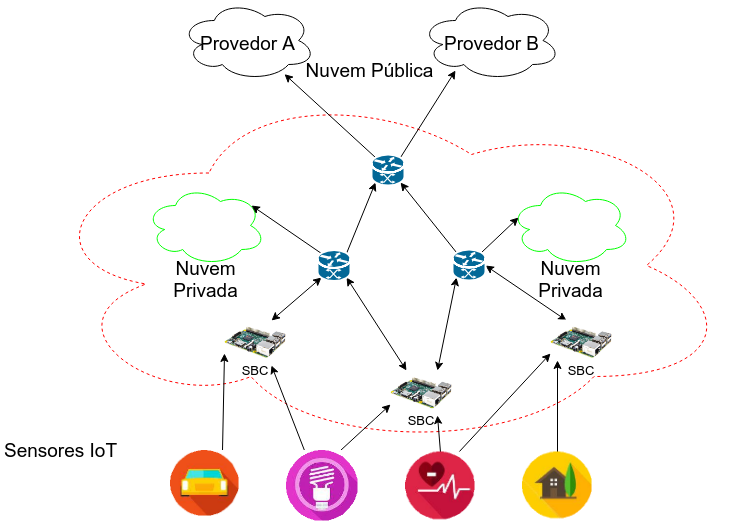
\includegraphics[width=0.8\textwidth]{figuras/idsa-iot-quali-000.png}
%   \caption{Estrutura Física da Arquitetura \arch.
%   Produzida e traduzida por \citeonline{Cassales2019}.}
%   \label{fig:ids-iot-phy}
%   \end{figure}
% \end{frame}

\end{document}
